\documentclass[UTF8, xcolor=table]{beamer}

% 定义本文所使用宏包
% !Mode:: "TeX:UTF-8"

% 原作者信息Original Authors:
% 张井   Jing Zhang: prayever@gmail.com     天津大学2010级管理与经济学部信息管理与信息系统专业硕士生
% 余蓝涛 Lantao Yu: lantaoyu1991@gmail.com  天津大学2008级精密仪器与光电子工程学院测控技术与仪器专业本科生

% Thanks 中大移植版by林海涛&徐浩晖&

%%%%%%%%%% Package %%%%%%%%%%%%

% 支持插图处理
\usepackage{graphicx}
% 控制文档布局
%\usepackage[a4paper,text={146.4 true mm,239.2 true mm},top= 26.2 true mm,left=31.8 true mm,head=6 true mm,headsep=6.5 true mm,foot=16.5 true mm]{geometry}
\usepackage[a4paper,text={146.4 true mm,239.2 true mm},top= 26.2 true mm,left=31.8 true mm,head=6 true mm,headsep=6.5 true mm,foot=16.5 true mm,footnotesep=-8 true mm]{geometry}

% 支持版面尺寸设置
% 支持国际标准单位
\usepackage[squaren]{SIunits}               

\usepackage{titletoc}                       % 控制目录的宏包
\usepackage[raggedleft]{titlesec}               % 控制标题的宏包

\usepackage{fancyhdr}                       % fancyhdr宏包 支持页眉和页脚的相关定义

\usepackage[UTF8]{ctex}                     % 支持中文显示
\usepackage{color}                          % 支持彩色
\usepackage{amsmath}                        % AMSLaTeX宏包 用来排出更加漂亮的公式
\usepackage{amssymb}                        % 数学符号生成命令
\usepackage[below]{placeins}    %允许上一个section的浮动图形出现在下一个section的开始部分,还提供\FloatBarrier命令,使所有未处理的浮动图形立即被处理
\usepackage{multirow}                       % 使用Multirow宏包,使得表格可以合并多个row格
\usepackage{booktabs}                       % 表格,横的粗线;\specialrule{1pt}{0pt}{0pt}
\usepackage{longtable}                      % 支持跨页的表格。
\usepackage{tabularx}                       % 自动设置表格的列宽
\usepackage{diagbox}						% 制作斜线单元格
\usepackage{makecell}

%\usepackage{subfigure}                      % 支持子图 %centerlast 设置最后一行是否居中
%\usepackage[subfigure]{ccaption}            % 支持子图的中文标题
% use the more updated subcaption package, which has replaced subfigure
\usepackage{subcaption}
%\usepackage{caption}
%\usepackage{capt-of}

\usepackage[sort&compress,numbers]{natbib}  % 支持引用缩写的宏包
\usepackage{enumitem}                       % 使用enumitem宏包,改变列表项的格式
\usepackage{calc}                           % 长度可以用+ - * / 进行计算
\usepackage{txfonts}                        % 字体宏包
\usepackage{bm}                             % 处理数学公式中的黑斜体的宏包
\usepackage[amsmath,thmmarks,hyperref]{ntheorem}  % 定理类环境宏包,其中 amsmath 选项用来兼容 AMS LaTeX 的宏包
\usepackage{CJKnumb}                        % 提供将阿拉伯数字转换成中文数字的命令
\usepackage{indentfirst}                    % 首行缩进宏包
%\usepackage{hypbmsec}                      % 用来控制书签中标题显示内容
\newcommand{\tabincell}[2]{\begin{tabular}{@{}#1@{}}#2\end{tabular}}
\usepackage{xcolor}
% 支持代码环境
\usepackage{listings}
\lstset{numbers=left,
	language=[ANSI]{C},
	numberstyle=\tiny,
	extendedchars=false,
	showstringspaces=false,
	breakatwhitespace=false,
	breaklines=true,
	captionpos=b,
	keywordstyle=\color{blue!70},
	commentstyle=\color{red!50!green!50!blue!50},
	frame=shadowbox,
	rulesepcolor=\color{red!20!green!20!blue!20}
}
% 支持算法环境
%\usepackage[boxed,ruled,lined]{algorithm2e}
%\usepackage{algorithmic}
\usepackage{algorithm,algpseudocode}

\usepackage{array}
\newcommand{\PreserveBackslash}[1]{\let\temp=\\#1\let\\=\temp}
\newcolumntype{C}[1]{>{\PreserveBackslash\centering}p{#1}}
\newcolumntype{R}[1]{>{\PreserveBackslash\raggedleft}p{#1}}
\newcolumntype{L}[1]{>{\PreserveBackslash\raggedright}p{#1}}

% 生成有书签的 pdf 及其生成方式。通常可以在 tjumain.tex 文件的第一行选择 pdflatex 或者是 dvipdfmx 编译手段。如果选择前者,则使用 pdflatex + pdflatex 编译; 如果选择后者,在编译的时候选择 latex + bibtex + latex + latex 编译。出现混淆的时候,系统会报错。
% 如果您的pdf制作中文书签有乱码使用如下命令,就可以解决了
\def\atemp{dvipdfmx}\ifx\atemp\usewhat
\usepackage[dvipdfmx,unicode,               % dvipdfmx 编译, 加入了中文复制,粘贴支持引擎。
            pdfstartview=FitH,
            bookmarksnumbered=true,
            bookmarksopen=true,
            colorlinks=false,
            pdfborder={0 0 1},
            citecolor=blue,
            linkcolor=red,
            anchorcolor=green,
            urlcolor=blue,
            breaklinks=true
            ]{hyperref}
\fi

\def\atemp{pdflatex}\ifx\atemp\usewhat
\usepackage{cmap}                           % pdflatex 编译时,可以生成可复制、粘贴的中文 PDF 文档, 缺点是在Windows上显示时效果不大好,字体发虚
\usepackage[pdftex,unicode,
            %CJKbookmarks=true,
            bookmarksnumbered=true,
            bookmarksopen=true,				
            hidelinks
%            colorlinks=true,		% original false
%            pdfborder={0 0 1},
%            citecolor=black,		% original blue
%            linkcolor=black,		% original red
%            anchorcolor=black,		% original green
%            urlcolor=blue,
%            breaklinks=false		% original true
            ]{hyperref}
\fi

% 新增for url
\usepackage{url}

% \pdfbookmark and \tableofcontents
\usepackage[bookmarks=true]{hyperref}
\usepackage{bookmark}

% xeCJK直接使用Window系统字体(一定要保证tex所存格式为UTF8,否则xeCJK汉字不显示)
\usepackage{xeCJK}

\usepackage{etoolbox}

% 控制打印模式
\usepackage{ifthen}
% 脚注跨章连续编号
%\usepackage{chngcntr}
% 脚注按页单独编号
\usepackage[perpage]{footmisc}

\graphicspath{{./figures/}}

\begin{document}
	\setbeamerfont{footnote}{size=\tiny}
	\setbeamerfont{caption}{size=\scriptsize}
	\setbeamertemplate{caption}[numbered]
	\setbeamerfont{subsection in toc}{size=\footnotesize}
	\renewcommand*{\bibfont}{\footnotesize}
	
	\title[融合长短记忆神经网络与卷积特征学习的图像语义分割]{中文题目 \\ \vskip 8pt \normalsize The English Title \\ Title...}
	\author[~~~~陈胜杰~~~~CHEN Shengjie]{}
	\institute[中山大学~数据科学与计算机学院~工程硕士(软件工程)]{}
	\date{}
	
	%% make title %%
	{
		\setbeamertemplate{headline}{}
		\setbeamertemplate{footline}{}
		
		\usebackgroundtemplate{%
			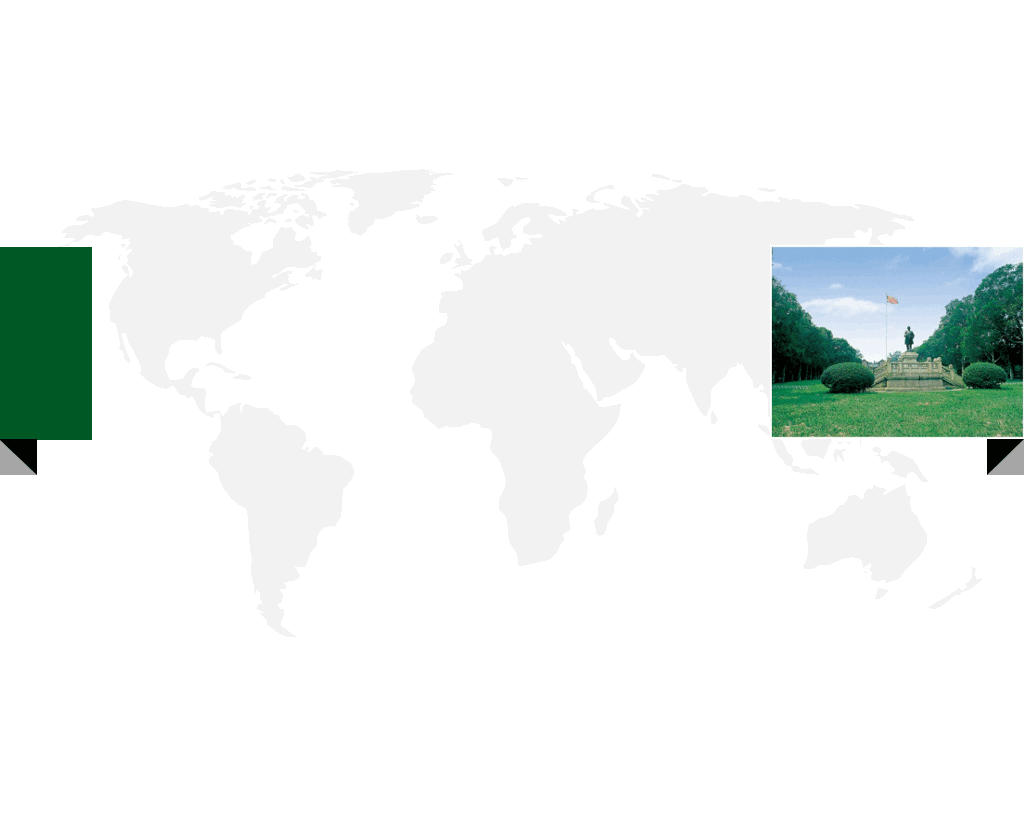
\includegraphics[width=\paperwidth,height=\paperheight]{styles/title.png}
		}
		
		\begin{frame}
		%\begin{frame}[plain]
			%% make logo without name %%
			%\begin{flushright}
			%	\vspace{-15mm}
			%	
\includegraphics[width=1.48cm]{styles/badge.png}
			%\end{flushright}
			
			%% make logo with name %%
			\begin{flushright}
				\vspace{-13.888mm}
				
\includegraphics[width=4.5cm]{styles/logo.png}
			\end{flushright}
		
			\vspace{-7.888mm}
			\titlepage
			
			\begin{flushright}
				\begin{tabular}{lc}
					学位申请人   &  \underline{\makebox[108pt][c]{陈胜杰}} \\
					专\ 业\ 名\ 称   &  \underline{\makebox[108pt][c]{工程硕士(软件工程)}} \\
					答\ 辩\ 时\ 间   &  \underline{\makebox[108pt][c]{May 13, 2018}} \\
				\end{tabular}
			\end{flushright}
		\end{frame}
	}
	\addtocounter{framenumber}{-1}
	
	%% make contents %%
	\frame {
		\frametitle{目录}
		\tableofcontents[sections={<1-7>}]
	}

	%% make body %%
	% !Mode:: "TeX:UTF-8"

\chapter{引言}
\label{ch:intro}

根据天津大学模板修改的符合中山大学毕业论文(至少是硕士论文)要求的Latex模板。

\section{使用方法}
\label{sec:usage}

本模板只包括内容方面的设计预定义,编译自行解决。作者使用的是Windows环境下MikTex+TeXstudio的组合。

\section{使用建议}
\label{sec:tips}

\subsection{普适问题}
\label{subsec:common}

普遍适用的论文排版问题:

\begin{itemize}
\item 图片标题在下,表格在上;一定要有标题,不能只是图1-1;与文字内容的间隔自行把握。
\item 参考文献建议使用.bib文件;也有使用Google Scholar的引用的,但有指出当中的“//”不符合规范。
\item 部分评审反馈,目录不包含摘要及目录本身,请根据情况自行斟酌。
\item 打印时需要右边翻页的问题(每章开始在右边页),可以在生成pdf后通过插入空白页解决(这样插入不会改变页码);或者尝试设置openright(未测试,有待探讨)。
\end{itemize}

\subsection{细节问题}
\label{subsec:specs}

一些细节的问题建议:
\begin{itemize}
\item 每个章节都有label,key使用ch:intro形式,以下使用sec:background等。图片key可以参考fig:scenes,表格参考tab:exp。
\item 图片、表格尽量在页的顶部,即float优先选择t。
\item 另外,为了打印时彩打方便,可以把需要彩打的图片尽量排版在一页,不过比较难调。
\item 虽然每个body的tex文件中包含了!Mode:: ``TeX:UTF-8"在文件开头,但仍有必要在IDE中将新建的tex文件设为UTF-8编码,否则可能无法正常显示中文。
\end{itemize}

\subsection{其他说明}
\label{sec:setting}

参考文献\cite{wu2013online}目前采用上标表示。使用cite命令。

目前页眉设置:每章第一页页眉只有中间的“中山大学硕士毕业论文”,后续页左边显示“中山大学硕士毕业论文”,右边显示“第n章”。

目前页脚设置:仅包含页码,居中,无横线。

参考文献和附录计算页数,包含在目录,页眉设置同每章第一页。正文前的部分无页眉。

\section{例子}
\label{sec:examples}

图例子。label要在caption后。多图或子图方法上网查吧。

\begin{figure}[!t]
	\centering
	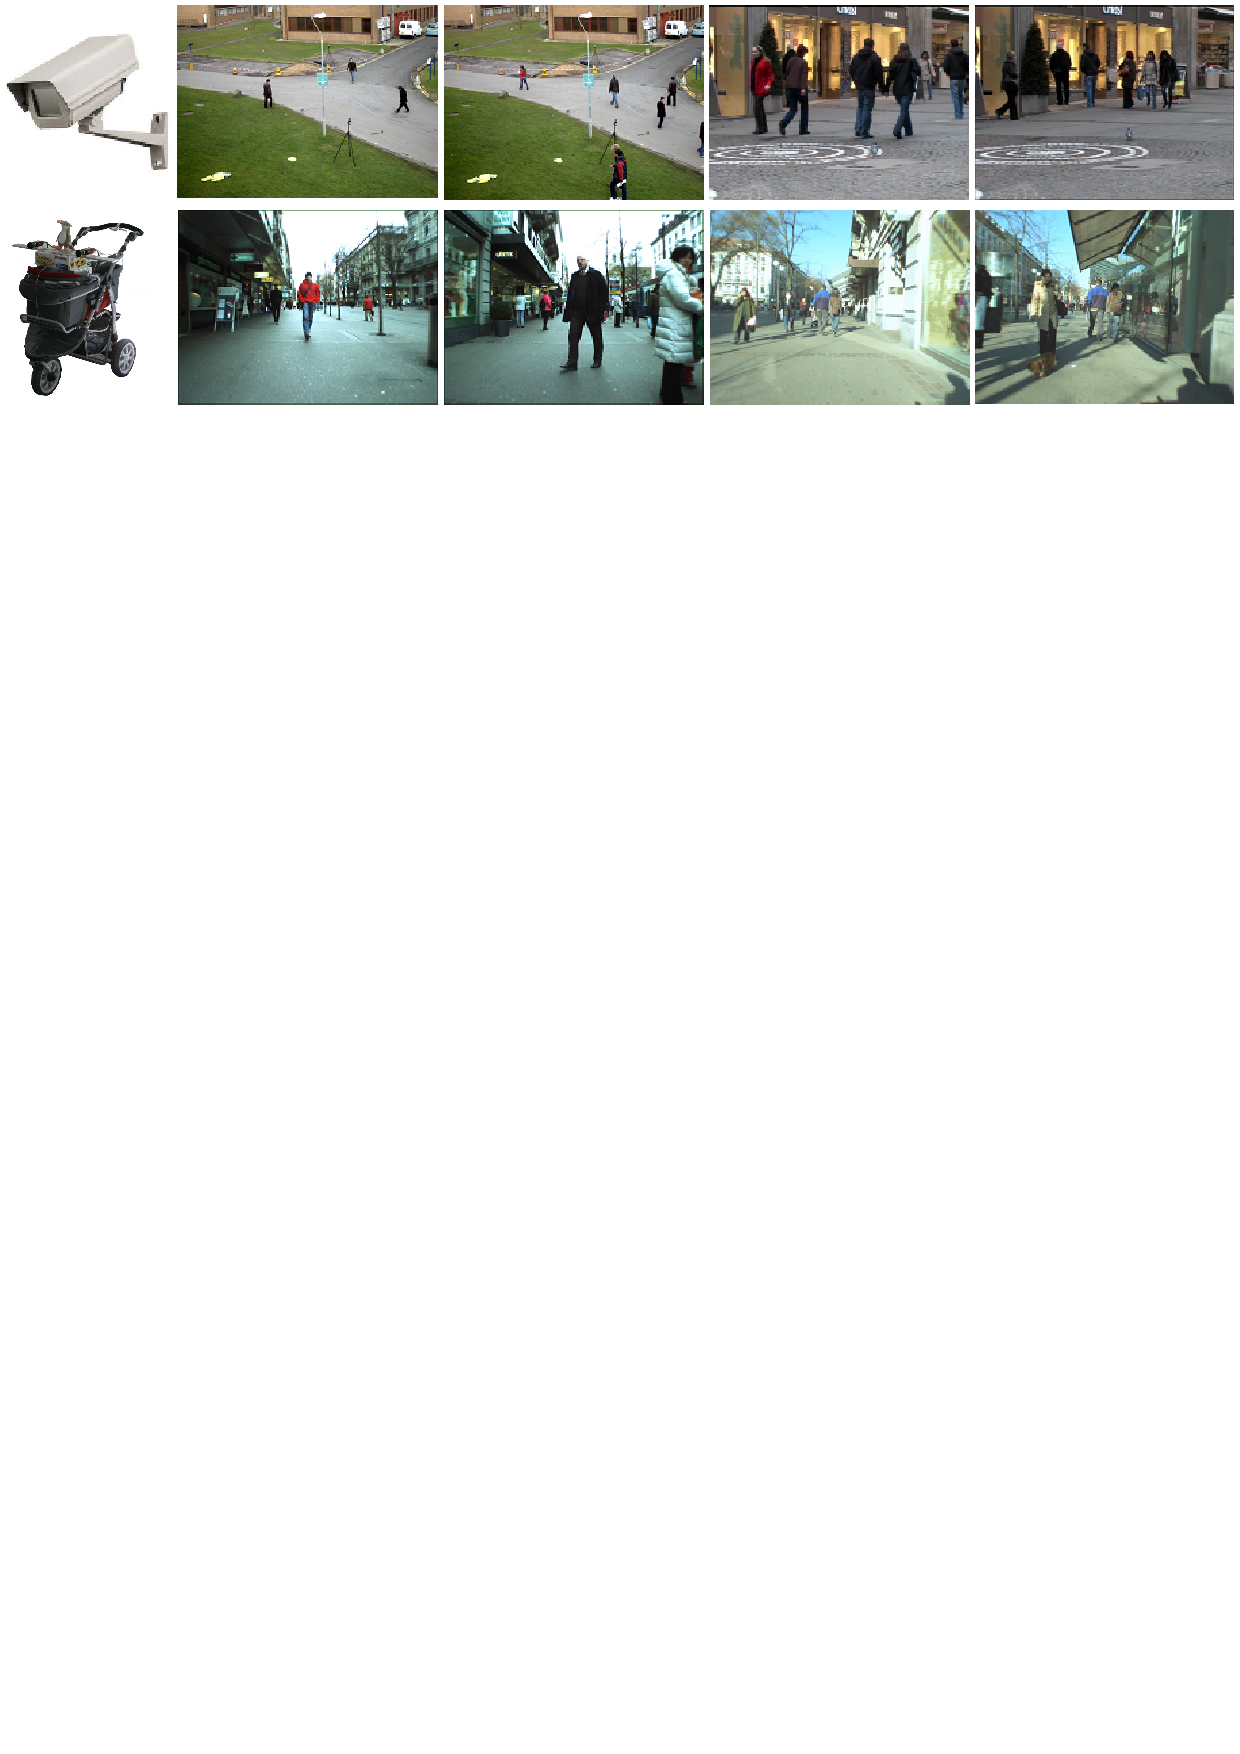
\includegraphics[width=0.95\textwidth]{scenes}
	\caption{图例}
	\label{fig:scenes}
\end{figure}

表例子。推荐使用这种三行表。缺省值使用三个“-”产生长横线“---”。

\begin{table}[!t]
\caption{示例表}
\label{tab:eg}
\vspace{0.5em}
\centering
\wuhao
	\begin{tabular}{ccccc}
	\toprule[1.5pt]
	表头 & 栏1 & 栏2 & 栏3 & 栏4 \\
	\midrule[1pt]
	内容1 & b & --- & $768 \times 576$ & 19 \\
	内容1 & a & 240/7 & $768 \times 576$ & --- \\
	\bottomrule[1.5pt]
	\end{tabular}
\end{table}

公式例子,与普通Latex数学公式无异。

\begin{equation}
1+1=2
\end{equation}

\section{章节安排}


	\section{深度神经网络}

\frame
{
  	\frametitle{\secname~ }
  	\begin{block}{前馈神经网络}
	  	传统的人工神经网络
  	\end{block}
  	\begin{block}{卷积神经网络}
	  	目前最为流行的,广泛应用于视觉任务的神经网络
  	\end{block}
  	\begin{block}{长短记忆网络}
	  	与卷积网络相比,更适用于处理时序信号
  	\end{block}
}

\subsection*{前馈神经网络结构}
\frame{
	\frametitle{}
    \begin{columns}[onlytextwidth]
		\begin{column}{0.5\textwidth}
			\vspace{-1.5em}
		\begin{itemize}
			\item 有向无环图的结构
			\item 输入层(数据特征)
			\item 隐含层(映射后的特征)
			\item 输出层(预测结果)
			\item 反向传播算法(训练方法)
		\end{itemize}
		\end{column}
		\begin{column}{0.5\textwidth}
		\begin{figure}[h] %structure of LSTM
	\centering
	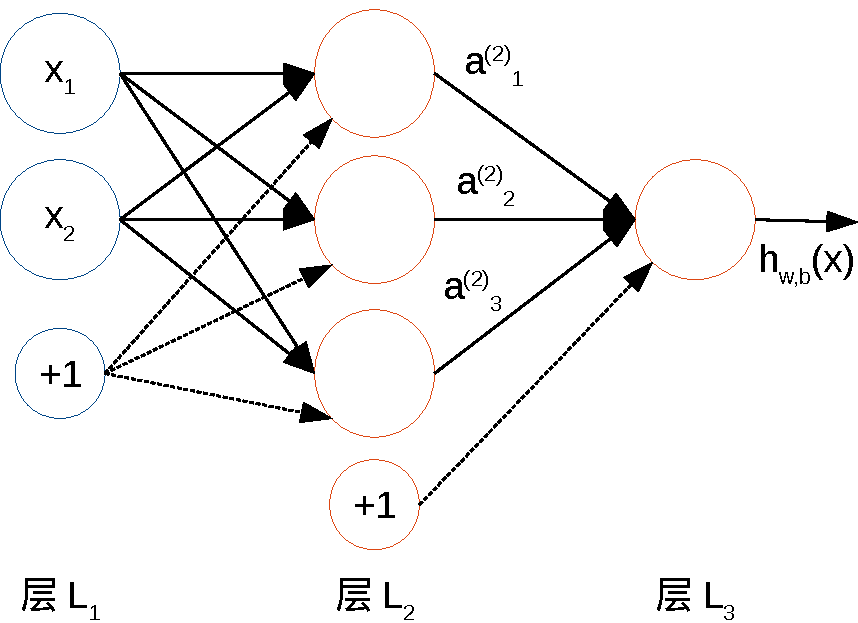
\includegraphics[width=0.9\textwidth]{demo_images/illustration/network1.pdf}
	\caption{前馈神经网络模型示意图}
	\label{fig:lstm}
\end{figure}
		\end{column} 
	\end{columns}
}

\subsection*{卷积神经网络}
\frame{
   	\frametitle{}
   	\vspace{-0.8em}
	\begin{figure}
	\centering
	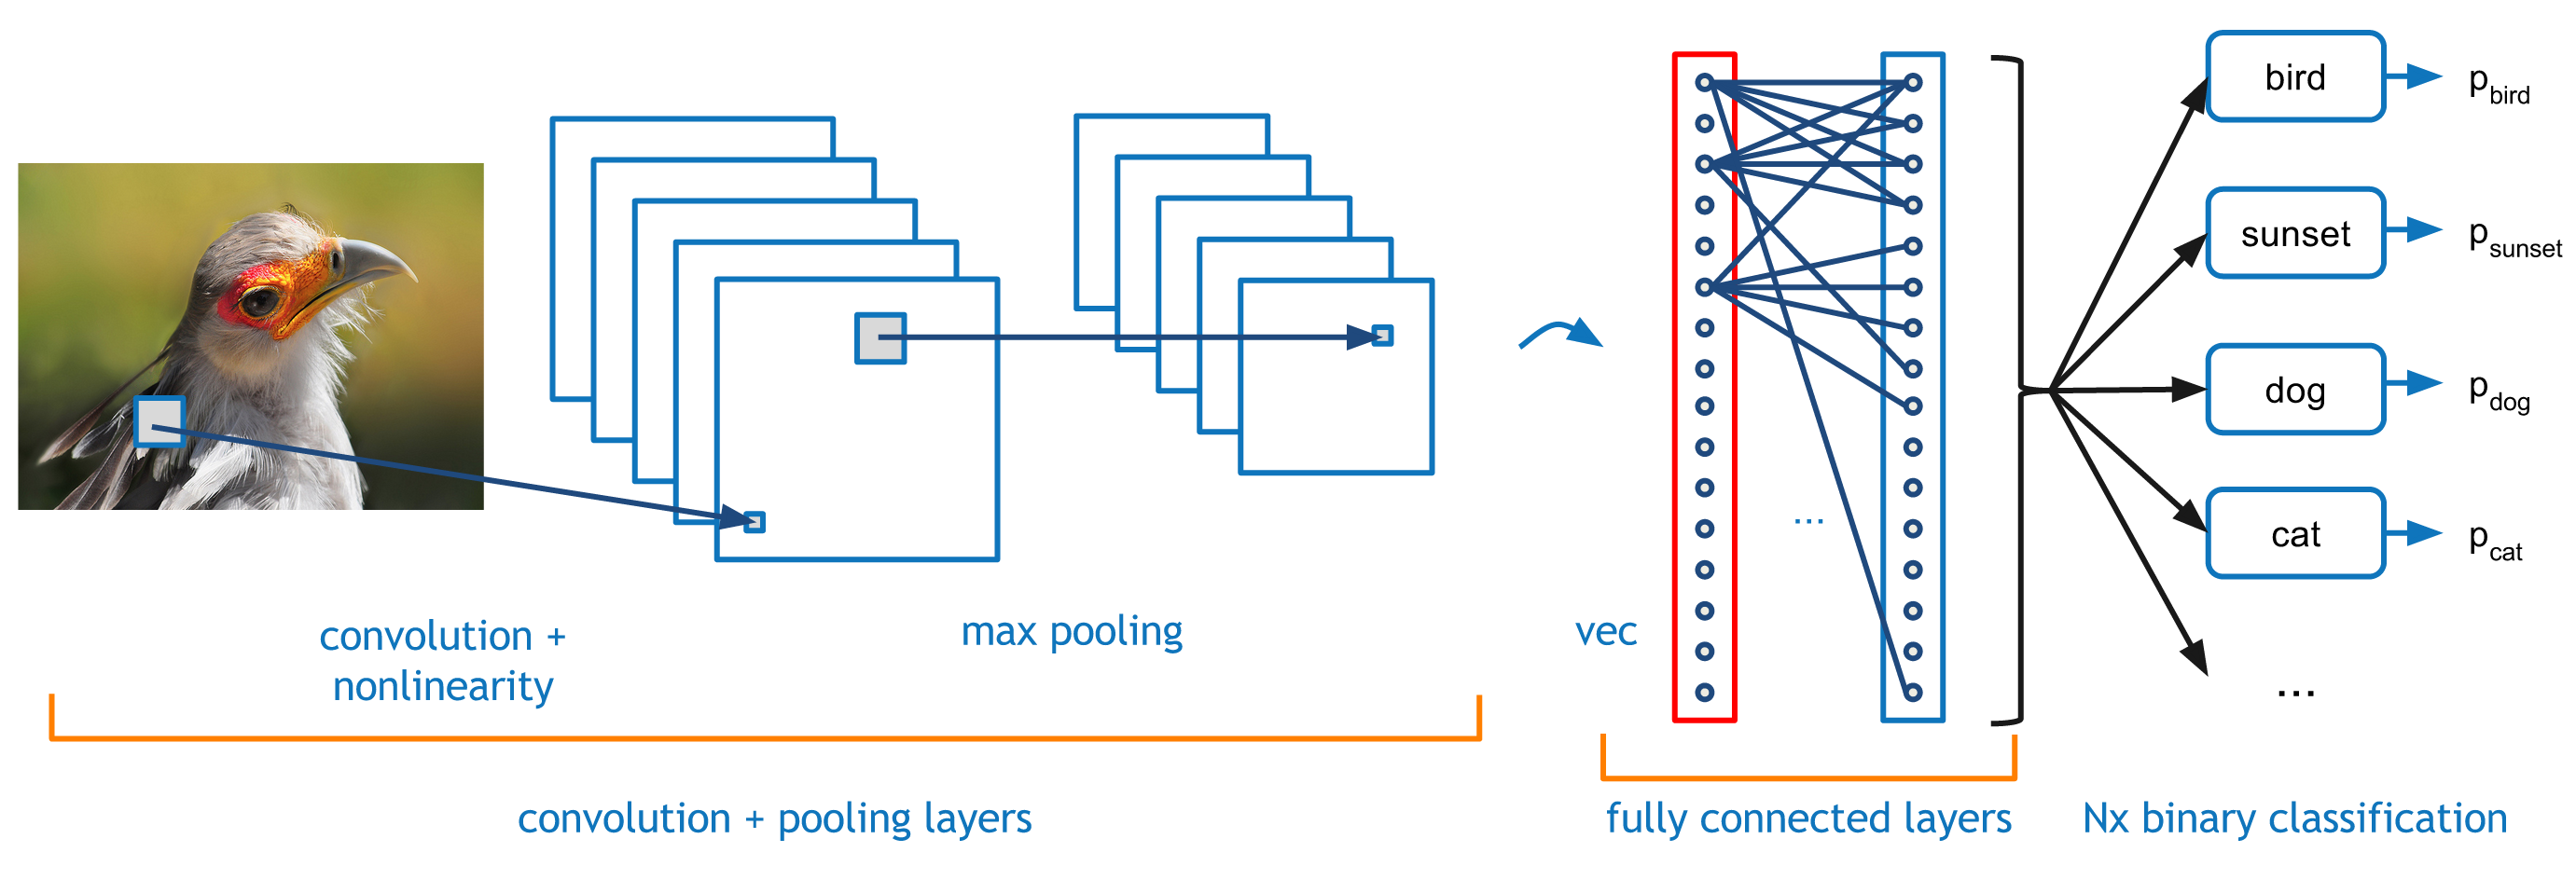
\includegraphics[width=0.8\textwidth]{demo_images/CNN}
	\caption{卷积网络模型示意图}
	\label{fig:network1}
\end{figure}
   	\vspace{-0.8em}
	\begin{block}{与前馈神经网络的区别}
	\begin{itemize}
		\item 直接作用于二维图像,无需特征设计阶段
		\item 卷积层,池化层
		\item 局部感知域,权重共享
	\end{itemize}
	\end{block}
}

\subsection*{长短记忆网络(处理一维信号)}
\frame{
	\frametitle{}
	\tiny
	\vspace{-2em}
    \begin{columns}[onlytextwidth]
        \begin{column}{0.5\textwidth}
	    \begin{figure}[h] %structure of LSTM
   	\centering
   	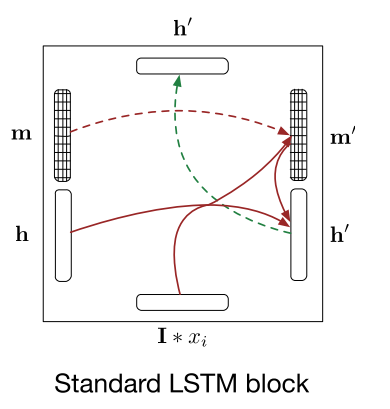
\includegraphics[width=0.6\textwidth]{demo_images/lstmblock1}
   	\caption{长短记忆网络区块示意图}
   	\label{fig:lstm}
\end{figure}
		\end{column} 
		%%%%%%% new column
		\begin{column}{0.5\textwidth}
			\begin{boxedminipage}{0.8\textwidth}
			\vspace{-1.5em}
			\begin{align}
				\label{eq:lstm}
				\begin{split}
				\textbf{g}^u &= \delta(\textbf{W}^u*\textbf{H}) \\
				\textbf{g}^f &= \delta(\textbf{W}^f*\textbf{H}) \\
				\textbf{g}^o &= \delta(\textbf{W}^o*\textbf{H}) \\
				\textbf{g}^c &= \mbox{tanh}(\textbf{W}^c*\textbf{H}) \\
				\textbf{m}' &= \textbf{g}^f \odot \textbf{m} + \textbf{g}^u \odot \textbf{g}^c \\
				\textbf{h}' &= \mbox{tanh}(\bf{g}^o \odot \bf{m}') \\
					\textbf{H} & = \begin{bmatrix}
					I*\textbf{x}_i \\ \textbf{h}
					\end{bmatrix}
			\end{split}
			\end{align}
		\end{boxedminipage}
		\end{column}
    \end{columns}
	
	\vspace{-1em}
	\begin{block}{缩写形式}
	\footnotesize
	\begin{equation*}
		(\textbf{h}', \textbf{m}') = \mbox{LSTM}\bigr(\textbf{H},\textbf{m},\textbf{W} \bigr)
	\end{equation*}
	其中\textbf{W}包含了四个门权值矩阵$\textbf{W}^u,\textbf{W}^f,\textbf{W}^o,\textbf{W}^c$。
	\end{block}
}

\subsection*{网格型长短记忆网络(处理N维信号)}
\frame{
	\frametitle{}
	\vspace{-1.5em}
	\begin{figure}[h]
	\centering
	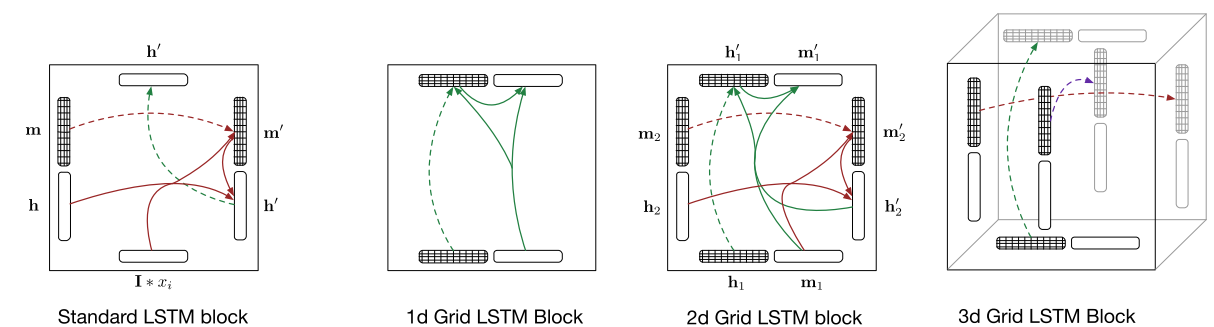
\includegraphics[width=\textwidth]{demo_images/gridlstm}
	\caption{网格型长短记忆网络区块示意图[Kalchbrenner et al, Grid LSTM, ICLR 2016]}
\end{figure}
	\vspace{-2em}
	\begin{block}{网格型长短记忆网络更新过程}
	\tiny
	\begin{columns}[onlytextwidth]
		\begin{column}{0.4\textwidth}
		\vspace{-0.5em}
			\begin{equation}
				\textbf{H} = \begin{bmatrix}
					\textbf{h}_i \\ \vdots \\ \textbf{h}_N
				\end{bmatrix}
			\end{equation}
		\end{column}
		\begin{column}{0.6\textwidth}
		\vspace{-1em}
			\begin{align}
				\begin{split}
				(\textbf{h}_1', \textbf{m}_1') & =  \mbox{LSTM}(\textbf{H}, \textbf{m}_1, \textbf{W}_1) \\ &\mbox{ }\vdots \\
				(\textbf{h}_N', \textbf{m}_N') & =  \mbox{LSTM}(\textbf{H}, \textbf{m}_N, \textbf{W}_N)
				\end{split}
				\label{eq:gridlstm}
			\end{align}
		\end{column}
	\end{columns}
	\end{block}
}
\endinput

	\section{网络模型结构}

\subsection*{网络整体结构}
\frame{
	\begin{figure}[h]
	\centering
	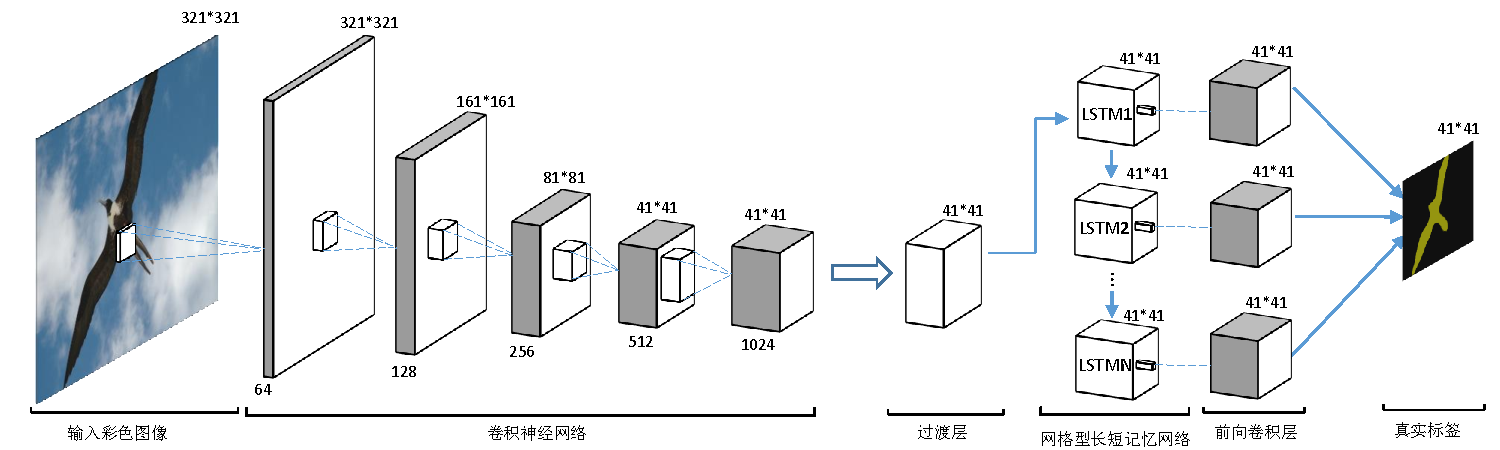
\includegraphics[width=0.9\textwidth,height=0.28\textwidth]{demo_images/illustration/networkstructure.pdf}
	\caption{网络整体结构图}
	\label{fig:networkstructure}
\end{figure}
	\vspace{-1em}
	\small
	\begin{block}{}
	\begin{itemize}
		\item  四个组成部分:\textbf{卷积网络部分},过渡层,\textbf{网格型长短记忆网络部分},前向卷积层
		\item 核心思想:在卷积网络后堆叠多层网格型长短记忆层
	\end{itemize}
	\end{block}
}

\subsection*{卷积网络部分}
\frame{
	\frametitle{}
	\vspace{-1em}
	\footnotesize
	\begin{block}{}
	\begin{itemize}
		\item 基于$VGG_{16}$模型\footnote{Simonyan \& Zissermanet, Very deep Convolutional Networks For Large-scale Image Recognition, ICLR 2015}, 含有16层卷积层
		\item 使用了“孔算法”,在不损失精度的情况下将模型参数减少了 6.5 倍\footnote{Chen et al, DeepLab-LargeFOV, ICLR 2015}
	\end{itemize}
	\end{block}
	\vspace{-1em}
	\begin{figure}[h]
	\centering
	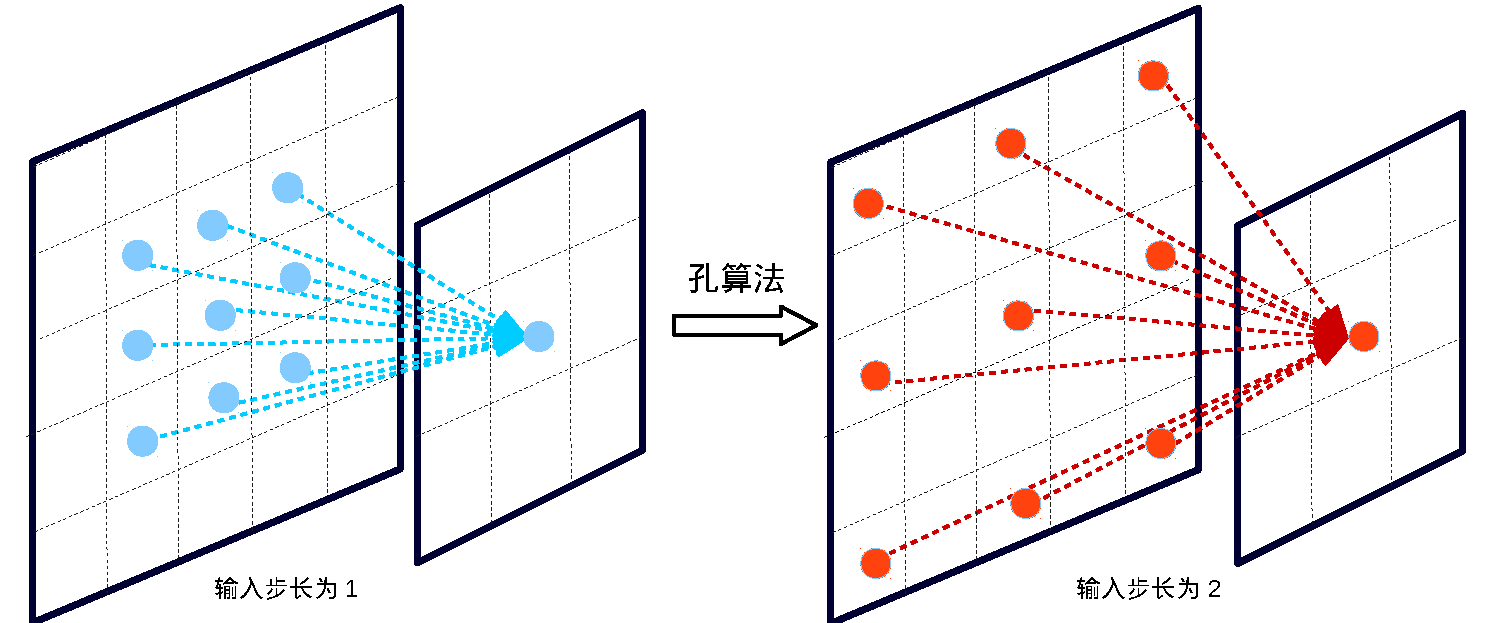
\includegraphics[width=0.7\textwidth]{demo_images/illustration/hole.pdf}
	\caption{"孔算法"示意图}
\end{figure}
}


\subsection*{网格型长短记忆网络部分}
\frame{
	\frametitle{}
	\vspace{-1em}
    \begin{columns}%[onlytextwidth]
        \begin{column}{0.6\textwidth}
        \vspace{0.2em}
		\begin{figure}
	\centering
	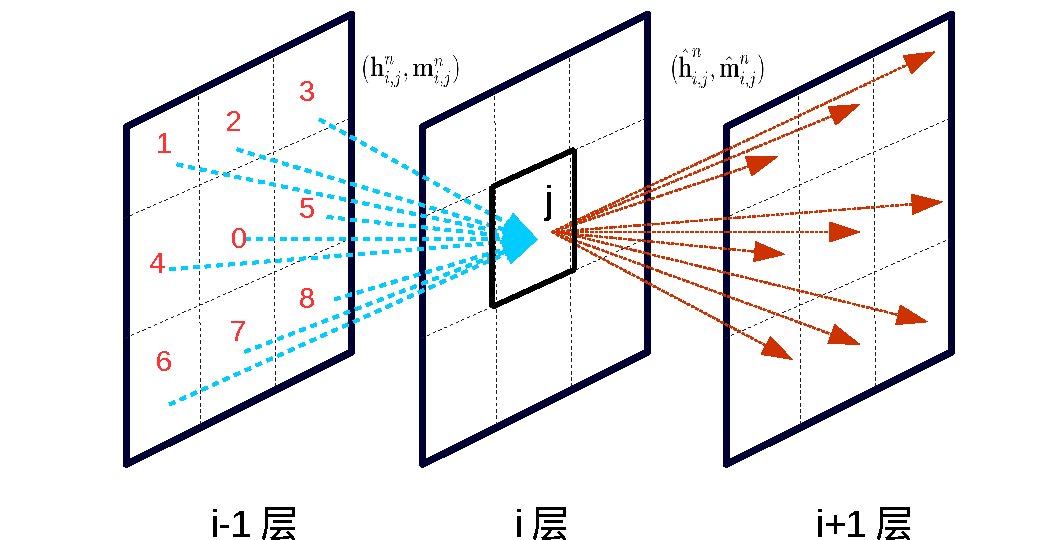
\includegraphics[width=\textwidth]{demo_images/illustration/neighboring.pdf}
	\caption{九维网格型长短记忆网络层之间的通信示意图}
	\label{fig:neighboring}
\end{figure}
		\end{column} 
		%%%%%%% new column
		\begin{column}{0.5\textwidth}
			\footnotesize
			\vspace{-1.5em}
			\begin{align}
				\begin{split}
				(\hat{\textbf{h}}_{i,j}^0,\hat{\textbf{m}}_{i,j}^0) &= \mbox{LSTM}(\textbf{H}_{i,j},\textbf{m}_{i,j}^0,\textbf{W}_i) \\
				(\hat{\textbf{h}}_{i,j}^1,\hat{\textbf{m}}_{i,j}^1) &= \mbox{LSTM}(\textbf{H}_{i,j},\textbf{m}_{i,j}^1,\textbf{W}_i) \\
				\vdots \\
				(\hat{\textbf{h}}_{i,j}^N,\hat{\textbf{m}}_{i,j}^N) &= \mbox{LSTM}(\textbf{H}_{i,j},\textbf{m}_{i,j}^N,\textbf{W}_i) \\
				\textbf{H}_{i,j} &= [\textbf{h}_{i,j}^0\mbox{ }\textbf{h}_{i,j}^1\mbox{ }...\mbox{ }\textbf{h}_{i,j}^N]^T
				\end{split}
			\end{align}
		\end{column}
    \end{columns}
	\footnotesize
	\vspace{-1em}
	\begin{block}{九维网格型长短记忆网络}
		\vspace{-0.7em}
		\begin{itemize}
			\item 每个位置的预测会受到上一层相邻八邻域特征的影响
			\item 随着层数的堆叠,每一位置将会有更大的感知域。
			\item 网格型长短记忆网络的层数通过实验来确定
		\end{itemize}
	\end{block}
}
	% !Mode:: "TeX:UTF-8"

\chapter{实验结果与分析}

也有另一种结构将相关研究放在第一章,从第二章开始讲述自己的研究。

\section{第一节}

呵呵

\subsection{第一节的第一小节}

哈哈

\subsection{第一节的第二小节}

嘿嘿

\section{第二节}

aa

\section{第三节}

\subsection{第二节的第一小节}

bb

\section{本章总结}

% 打印时插入必要的空白页
\ifprint
\newpage
\thispagestyle{empty}
\mbox{}

% 避免空白页影响页码编号
\clearpage
\setcounter{page}{10}
\fi
	% !Mode:: "TeX:UTF-8"

\chapter{相关研究}

也有另一种结构将相关研究放在第一章,从第二章开始讲述自己的研究。

\section{第一节}

呵呵

\subsection{第一节的第一小节}

哈哈

\subsection{第一节的第二小节}

嘿嘿

\section{第二节}

aa

\subsection{第二节的第一小节}

bb

\section{第三节}

\section{本章总结}

	\section{致谢}

\subsection*{}
\frame{
	\frametitle{致谢}
	\begin{block}{感谢每一个帮助过我的人}
	\begin{itemize}
		\item 首先要感谢的是我的指导老师的悉心指导
		\item 感谢师兄师姐、同学的帮助
		\item 感谢家人的支持
		\item 感谢答辩委员会的聆听和指导
	\end{itemize}
	\end{block}
	\vspace{-1em}
	\note{
		我的展示到此结束,我要感谢我的指导老师,师兄师姐同学,家人还有答辩委员会老师的聆听与指导。谢谢大家
	}
}
\frame{
	\frametitle{Q \& A}
	\begin{block}{Questions?}
	 ~\\ ~\\
	 \center{\Large{Thank you!}}
	 \\ ~\\ ~\\ ~\\ ~\\ 
	\end{block}
	\note{
		现在是问答时间。请问老师们对我的展示有什么疑问?
	}
}



\end{document}